
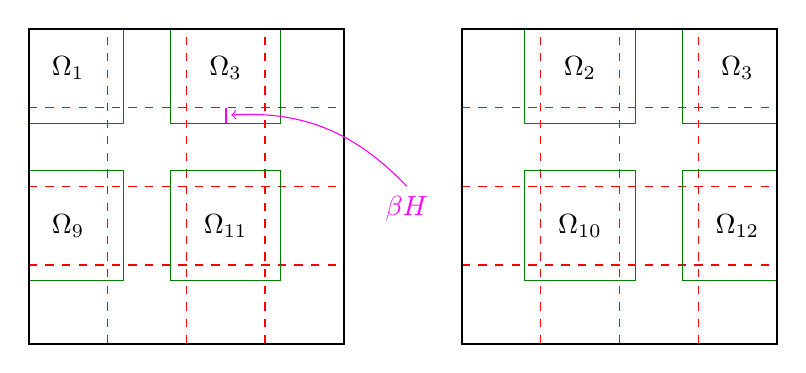
\begin{tikzpicture}
    \draw[dashed, red] (0, 0) grid (4,4);
    \draw[Green] (0, 4) rectangle (1.2, 2.8);
    \draw[Green] (1.8, 2.8) rectangle (3.2, 4);
    \draw[Green] (0, 2.2) rectangle (1.2, 0.8);
    \draw[Green] (1.8, 2.2) rectangle (3.2, 0.8);
    \draw[thick] (0, 0) rectangle (4, 4);
    \node[]() at (0.5, 3.5) {$\Omega_1$};
    \node[]() at (2.5, 3.5) {$\Omega_3$};
    \node[]() at (0.5, 1.5) {$\Omega_9$};
    \node[]() at (2.5, 1.5) {$\Omega_{11}$};

    \draw[thick, Magenta] (2.5, 2.8) -- (2.5, 3);

    \draw[<-, shorten <=2pt, Magenta] (2.5, 2.9) to[bend left=25](4.8, 2)
    node[below]{$\beta H$}
    ;
    \begin{scope}[xshift=5.5cm]
    \draw[dashed, red] (0, 0) grid (4,4);
    \draw[Green] (0.8, 4) rectangle (2.2, 2.8);
    \draw[Green] (2.8, 4) rectangle (4, 2.8);
    \draw[Green] (0.8, 2.2) rectangle (2.2, 0.8);
    \draw[Green] (2.8, 2.2) rectangle (4, 0.8);
    \draw[thick] (0, 0) rectangle (4, 4);
    \node[]() at (1.5, 3.5) {$\Omega_2$};
    \node[]() at (3.5, 3.5) {$\Omega_3$};
    \node[]() at (1.5, 1.5) {$\Omega_{10}$};
    \node[]() at (3.5, 1.5) {$\Omega_{12}$};
    \end{scope}
\end{tikzpicture}
